\documentclass[10pt,letterpaper]{article}
\usepackage[utf8]{inputenc}
\usepackage[english]{babel}
\usepackage{amsmath}
\usepackage{amsfonts}
\usepackage{amssymb}
\usepackage{graphicx}
\usepackage{verbatim}
\usepackage{listings}
\usepackage{color}
\usepackage{hyperref}
\usepackage[document]{ragged2e}

\usepackage{geometry}
\geometry{letterpaper, margin=1.0in}


\definecolor{mygreen}{rgb}{0,0.5,0}
\definecolor{mygray}{rgb}{0.9,0.9,0.9}
\definecolor{mymauve}{rgb}{0.58,0,0.82}


\lstset{ %
  backgroundcolor=\color{mygray},  % choose the background color; you must add \usepackage{color} or \usepackage{xcolor}
  basicstyle=\footnotesize,        % the size of the fonts that are used for the code
  breakatwhitespace=false,         % sets if automatic breaks should only happen at whitespace
  breaklines=true,                 % sets automatic line breaking
  captionpos=b,                    % sets the caption-position to bottom
  commentstyle=\color{mygreen},    % comment style
  deletekeywords={...},            % if you want to delete keywords from the given language
  escapeinside={\%*}{*)},          % if you want to add LaTeX within your code
  extendedchars=true,              % lets you use non-ASCII characters; for 8-bits encodings only, does not work with UTF-8
  frame=single,                    % adds a frame around the code
  keepspaces=true,                 % keeps spaces in text, useful for keeping indentation of code (possibly needs columns=flexible)
  keywordstyle=\color{blue},       % keyword style
  language=bash,                   % the language of the code
  otherkeywords={*,...},           % if you want to add more keywords to the set
  numbers=left,                    % where to put the line-numbers; possible values are (none, left, right)
  numbersep=5pt,                   % how far the line-numbers are from the code
  numberstyle=\tiny\color{mygray}, % the style that is used for the line-numbers
  rulecolor=\color{black},         % if not set, the frame-color may be changed on line-breaks within not-black text (e.g. comments (green here))
  showspaces=false,                % show spaces everywhere adding particular underscores; it overrides 'showstringspaces'
  showstringspaces=false,          % underline spaces within strings only
  showtabs=false,                  % show tabs within strings adding particular underscores
  stepnumber=2,                    % the step between two line-numbers. If it's 1, each line will be numbered
  stringstyle=\color{mymauve},     % string literal style
  tabsize=2,                       % sets default tabsize to 2 spaces
  title=\lstname                   % show the filename of files included with \lstinputlisting; also try caption instead of title
}







\author{Li Tai Fang / li\_tai.fang@roche.com}

\title{SomaticSeq Documentation}

\begin{document}

\maketitle



\begin{sloppypar}




\tableofcontents


% Need line for each paragraph:
\setlength{\parskip}{\baselineskip}


\section{Introduction} \label{Introduction}

SomaticSeq is a flexible post-somatic-mutation-calling algorithm for improved accuracy. It is compatible with 10+ somatic mutation callers. Any combination of them can be used to obtain a combined call set with sequencing features extracted into TSV and VCF files. In addition, SomaticSeq uses machine learning to distinguish true mutations from false positives from that call set. The mutation callers we have incorporated are MuTect/Indelocator/MuTect2 \cite{mutect}, VarScan2 \cite{varscan2}, JointSNVMix \cite{jointsnvmix2}, SomaticSniper \cite{somaticsniper}, VarDict \cite{vardict}, MuSE \cite{muse}, LoFreq \cite{lofreq}, Scalpel \cite{scalpel}, Strelka2 \cite{strelka2}, TNscope \cite{tnscope}, and Platypus \cite{platypus}. You may incorporate some or all of those callers into your own pipeline with SomaticSeq.


The manuscript, An ensemble approach to accurately detect somatic mutations using SomaticSeq, was published in \href{http://dx.doi.org/10.1186/s13059-015-0758-2}{Genome Biology 2015, 16:197} \cite{Fang_2015}. 
The SomaticSeq project is located at \href{https://github.com/bioinform/somaticseq}{\textit{https://github.com/bioinform/somaticseq}}. 
There have been some major improvements in SomaticSeq since that Genome Biology publication in 2015. 

The script somaticseq\_parallel.py can 1) train the call set into a classifier, 2) predict high-confidence somatic mutations from the call set based on a pre-defined classifier, or 3) default to consensus mode, i.e., extract sequencing features and output the TSV and VCF files, and then label the calls (i.e., PASS, LowQual, or REJECT) based on majority vote of the tools.



\subsection{Dependencies}

\begin{enumerate}

    \item
    SomaticSeq was written in \emph{Python 3} under Linux environment. In addition, Python libraries of \emph{numpy}, \emph{scipy}, and \emph{pysam} are also required. 

    \item
    SomaticSeq also uses \emph{BEDTools} \cite{bedtools} to manipulate bed file inputs, i.e., regions to include and/or exclude in the workflow. 

    \item
    \emph{R}, as well as \emph{ada} library (if you intend to use this).

    \item
    At its core, SomaticSeq combines and then filters the results of multiple somatic mutation detection algorithms based on many sequencing features. Generally speaking, at least one compatible caller needs to be run to generate a list of mutation candidates for SomaticSeq to evaluate. It is compatible with the following callers: the original MuTect/Indelocator as well as GATK4's Mutect2 \cite{mutect}, VarScan2 \cite{varscan2}, JointSNVMix2 \cite{jointsnvmix2}, SomaticSniper \cite{somaticsniper}, VarDict \cite{vardict}, MuSE \cite{muse}, LoFreq \cite{lofreq}, Scalpel \cite{scalpel}, Strelka2 \cite{strelka2}, TNscope \cite{tnscope}, and Platypus \cite{platypus}.  
    
    \item
    \emph{Docker} [\href{http://www.docker.com}{http://www.docker.com}] is a container technology that can be used to package softwares and their dependencies in a portable Docker images, which can be used to execute a workflow reproducibly across different platforms and environments. SomaticSeq does not require Docker \textit{per se}, but we have created Docker images of it, along with a number of compatible somatic mutation callers to make life easier for new users. The advantage of using container technologies like Docker, is that one does not necessarily have to create the right software environment with the correct dependencies for every software in a workflow, e.g,. by creating a Docker image for MuTect2, the users can simply use that Docker image for MuTect 2 tasks. Otherwise, they must make sure to have the correct Java version and others dependencies to run MuTect2, and that those dependencies do not conflict with other software that may need different Java versions. 

\end{enumerate}






\subsection{Docker images}

SomaticSeq and the somatic mutation callers that we routinely use were dockerized. 

\begin{itemize}

  \item SomaticSeq:    \href{https://hub.docker.com/r/lethalfang/somaticseq}{https://hub.docker.com/r/lethalfang/somaticseq}
  
  \item MuTect2:       \href{https://hub.docker.com/r/broadinstitute/gatk}{https://hub.docker.com/r/broadinstitute/gatk}

  \item VarScan2:      \href{https://hub.docker.com/r/djordjeklisic/sbg-varscan2}{https://hub.docker.com/r/djordjeklisic/sbg-varscan2}

  \item JointSNVMix2:  \href{https://hub.docker.com/r/lethalfang/jointsnvmix2}{https://hub.docker.com/r/lethalfang/jointsnvmix2}

  \item SomaticSniper: \href{https://hub.docker.com/r/lethalfang/somaticsniper}{https://hub.docker.com/r/lethalfang/somaticsniper}

  \item VarDict:       \href{https://hub.docker.com/r/lethalfang/vardictjava}{https://hub.docker.com/r/lethalfang/vardictjava}

  \item MuSE:          \href{https://hub.docker.com/r/marghoob/muse}{https://hub.docker.com/r/marghoob/muse}

  \item LoFreq:        \href{https://hub.docker.com/r/lethalfang/lofreq}{https://hub.docker.com/r/lethalfang/lofreq}

  \item Scalpel:       \href{https://hub.docker.com/r/lethalfang/scalpel}{https://hub.docker.com/r/lethalfang/scalpel}

  \item Strelka2:      \href{https://hub.docker.com/r/lethalfang/strelka}{https://hub.docker.com/r/lethalfang/strelka}

\end{itemize}



\section{Download and install SomaticSeq} \label{download_somaticseq}

Source code of SomaticSeq is available via Github repository in BSD 2-Clause open source license: \href{https://github.com/bioinform/somaticseq}{https://github.com/bioinform/somaticseq}. The latest source code can be cloned by the git command:
\begin{lstlisting}
git clone https://github.com/bioinform/somaticseq.git
\end{lstlisting}


To install SomaticSeq, then the core script \textit{somaticseq\_parallel.py} will be in your path. 
\begin{lstlisting}
./setup.py install
\end{lstlisting}


\section{How to run SomaticSeq} \label{Wrapper_script}

The \textit{somaticseq\_parallel.py} module calls a series of programs and procedures \textbf{after} you have run your individual somatic mutation callers. Section \ref{dockerized_callers} will teach you how to run those mutation callers that we have been dockerized. It also includes ways to create semi-simulated training data that can be used to create SomaticSeq classifiers. In the next section, we will describe the workflow in this wrapper script in detail. 

Both paired and single modes are supported, although single mode is not as well validated scientifically as the paired mode. To see the required and optional input files and parameters to \textit{somaticseq\_parallel.py}:

\begin{lstlisting}
# See the global input parameters
somaticseq_parallel.py --help

# Parameters for paired-sample mode (i.e., tumor-normal)
somaticseq_parallel.py paired --help

# Parameters for single-sample mode
somaticseq_parallel.py single --help
\end{lstlisting}


\subsection{SomaticSeq Training Mode} \label{somaticseq_train}

To create SomaticSeq classifiers, you need a VCF file containing true SNVs and a VCF file containing true INDELs, and invoke the training node with \emph{\texttt{--}somaticseq-train} flag. There is also an option to include a list of regions to include and/or exclude from this exercise. The exclusion or inclusion regions can be VCF or BED files. An inclusion region may be subset of the call sets where you have validated their true/false mutation status, so that only those regions will be used for training. An exclusion region can be regions where the ``truth'' is ambigious. All the variants in the truth VCF files are assumed to be true positives and will be labeled such. Every mutation call not in the truth VCF files is assumed to be false positives and will be labeled as such (as long as the genomic coordiante is in inclusion region and not in exclusion region if those regions are provided). 

All the VCF files from individual callers are optional, but you need at least one or there will be nothing to do. All VCF files can be bgzipped if they have .vcf.gz extensions. It is imperative that you will use the same parameter for prediction as you do for training. 


\begin{lstlisting}
somaticseq_parallel.py \
--output-directory     OUTPUT_DIR \
--genome-reference     GRCh38.fa \
--inclusion-region     genome.bed \
--exclusion-region     blacklist.bed \
--truth-snv            truePositives.snv.vcf \
--truth-indel          truePositives.indel.vcf \
--threads              28 \
--somaticseq-algorithm xgboost \
--somaticseq-train     \
paired                 \
--tumor-bam-file       tumor.bam \
--normal-bam-file      matched_normal.bam \
--mutect2-vcf          MuTect2.vcf \
--vardict-vcf          VarDict.vcf \
--muse-vcf             MuSE.vcf \
--strelka-snv          Strelka/results/variants/somatic.snvs.vcf.gz \
--strelka-indel        Strelka/results/variants/somatic.indels.vcf.gz
\end{lstlisting}


For the command's argument placement, caller output and bam files are input ``after'' \textit{paired} or \textit{single} option. Everything else goes before, e.g., reference, ground truths, resources such as dbSNP and COSMIC, etc. 

Parallel processing is achieved by splitting the inclusion BED file into a number of sub-BED files of equal region sizes, named 1.th.input.bed, 2.th.input.bed, ..., n.th.input.bed. Then each process will be run using each sub-BED file as the inclusion BED file. If there is no inclusion BED file in the command argument, it will split the reference.fa.fai file instead. 

SomaticSeq supports any combination of the somatic mutation callers we have incorporated into the workflow. SomaticSeq will run based on the output VCFs you have provided. It will train for SNV and/or INDEL if you provide the truePositives.snv.vcf and/or truePositives.indel.vcf file(s) and invoke the \textit{\texttt{--}somaticseq-train} option. Otherwise, it will fall back to the simple caller consensus mode.




\subsection{SomaticSeq Prediction Mode} \label{somaticseq_prediction}

Make sure the classifiers (.RData files) are supplied, Without either of them, or it will fall back to the simple caller consensus mode.

\begin{lstlisting}
# The *.RData files are trained classifier from the training mode.
somaticseq_parallel.py \
--classifier-snv       Ensemble.sSNV.tsv.xgb.v3.x.x.classifier \
--classifier-indel     Ensemble.sINDEL.tsv.xgb.v3.x.x.classifier \
--output-directory     OUTPUT_DIR \
--genome-reference     GRCh38.fa \
--inclusion-region     genome.bed \
--exclusion-region     blacklist.bed \
--somaticseq-algorithm xgboost \
--threads              12 \
paired                 \
--tumor-bam-file       tumor.bam \
--normal-bam-file      matched_normal.bam \
--mutect2-vcf          MuTect2/variants.vcf \
--vardict-vcf          VarDict/variants.vcf \
--muse-vcf             MuSE/variants.snp.vcf \
--strelka-snv          Strelka/variants.snv.vcf \
--strelka-indel        Strelka/variants.indel.vcf
\end{lstlisting}



\subsection{SomaticSeq Consensus Mode} \label{somaticseq_default_mode}

Same as the commands previously, but without including the classifiers (.RData files) or invoking \textit{--somaticseq-train}. Without those information, SomaticSeq will forgo machine learning, and fall back into a simple majority vote. The following is an example:

\begin{lstlisting}
# The *.RData files are trained classifier from the training mode.
somaticseq_parallel.py \
--output-directory  OUTPUT_DIR \
--genome-reference  GRCh38.fa \
--inclusion-region  genome.bed \
--exclusion-region  blacklist.bed \
--threads           12 \
paired              \
--tumor-bam-file    tumor.bam \
--normal-bam-file   matched_normal.bam \
--mutect2-vcf       MuTect2/variants.vcf \
--vardict-vcf       VarDict/variants.vcf \
--muse-vcf          MuSE/variants.snp.vcf \
--strelka-snv       Strelka/variants.snv.vcf \
--strelka-indel     Strelka/variants.indel.vcf
\end{lstlisting}







\section{SomaticSeq as a Python library} \label{somaticseq_package}


Section \ref{Wrapper_script} described how to use SomaticSeq as a software. It is also possible to treat SomaticSeq as a python library extension for your own software. So here we describe in detail the procedures and functions that make up SomaticSeq. 
 

\subsection{Module: somaticseq\_parallel.py} \label{module:somaticseq_parallel}

The \emph{somaticseq\_parallel.py} script simply calls for \emph{somaticseq/run\_somaticseq.py} module (Sec. \ref{module:run_somaticseq}), and parallelize the runs by splitting the input BED file into a number of equal-sized (in terms of total base pairs) regions. The BED file splitting is achieved by \emph{utilities/split\_Bed\_into\_equal\_regions.py} (Sec. \ref{module:split_bed}).


\subsection{Module: somaticseq/run\_somaticseq.py} \label{module:run_somaticseq}

The core module for SomaticSeq is \emph{somaticseq/run\_somaticseq.py}. It converts individual VCF files from somatic mutation caller(s) into SomaticSeq TSV and VCF files. There are two main functions in the module, \emph{runPaired} and \emph{runSingle}. Depending on the mode, either of them can be called. For example:

\begin{lstlisting}
  # Module is located somaticseq/somaticseq/run_somaticseq.py
  import somaticseq.somaticseq.run_somaticseq as run_somaticseq
  
  run_somaticseq.runPaired(outdir='/PATH/TO/SomaticSeq', ref='/PATH/TO/GRCh38.fa', tbam='/PATH/TO/tumor.bwa.bam', nbam='/PATH/TO/normal.bwa.bam', tumor_name='TUMOR', normal_name='NORMAL', truth_snv=None, truth_indel=None, classifier_snv=None, classifier_indel=None, pass_threshold=0.5, lowqual_threshold=0.1, hom_threshold=0.85, het_threshold=0.01, dbsnp='/PATH/TO/dbSNP_138.hg38.vcf.vcf', cosmic='/PATH/TO/COSMIC.v85.vcf', inclusion='/PATH/TO/Exon_Capture.bed', exclusion='/PATH/TO/ignore.bed', mutect=None, indelocator=None, mutect2='/PATH/TO/MuTect2.vcf', varscan_snv=None, varscan_indel=None, jsm=None, sniper=None, vardict='/PATH/TO/VarDict.vcf', muse='/PATH/TO/MuSE.vcf', lofreq_snv='/PATH/TO/LoFreq.snv.vcf.gz', lofreq_indel='/PATH/TO/LoFreq.indel.vcf.gz', scalpel=None, strelka_snv='/PATH/TO/Strelka/results/variants/somatic_ssnv.vcf.gz', strelka_indel='/PATH/TO/Strelka/results/variants/somatic_sindel.vcf.gz', tnscope=None, platypus=None, min_mq=1, min_bq=5, min_caller=0.5, somaticseq_train=False, ensembleOutPrefix='Ensemble.', consensusOutPrefix='Consensus.', classifiedOutPrefix='SSeq.Classified.', algo='ada', keep_intermediates=False)
\end{lstlisting}

The parameters of \emph{ensembleOutPrefix}, \emph{consensusOutPrefix}, and \emph{classifiedOutPrefix} will dictate the output file names under outdir.


We'll briefly describe the procedures of runPaired here. First of all, the \emph{somaticseq/combine\_callers.py} module (combinePaired function) will combine all the input VCF files into two minimal VCF files, one for SNVs and one for INDELs, that include each unique variant call. These VCF files serve as input files for the next steps, where features are extracted from each of the variant and then converted to the SomaticSeq TSV files by the \emph{somaticseq/somatic\_vcf2tsv.py} module (Sec. \ref{module:vcf2tsv}).

If training mode was invoked (Sec. \ref{somaticseq_train}), SomaticSeq classifiers would be built (Sec. \ref{module:r_train}). If prediction mode was invoked, an additional TSV file with prediction scores will be created (Sec. \ref{module:r_predict}). 

Finally, the TSV files will be converted to SomaticSeq VCF file output by somaticseq/SSeq\_tsv2vcf.py (Sec. \ref{module:vcf2tsv}). 



Likewise, the single sample mode to convert various individual VCF outputs would be something like this:

\begin{lstlisting}
  import somaticseq.somaticseq.run_somaticseq as run_somaticseq
  
  run_somaticseq.runSingle(outdir='/PATH/TO/SomaticSeq', ref='/PATH/TO/GRCh38.fa', bam='/PATH/TO/tumor.bwa.bam', tumor_name='TUMOR', truth_snv=None, truth_indel=None, classifier_snv=None, classifier_indel=None, pass_threshold=0.5, lowqual_threshold=0.1, hom_threshold=0.85, het_threshold=0.01, dbsnp='/PATH/TO/dbSNP_138.hg38.vcf.vcf', cosmic='/PATH/TO/COSMIC.v85.vcf', inclusion='/PATH/TO/Exon_Capture.bed', exclusion='/PATH/TO/ignore.bed', mutect=None, mutect2='/PATH/TO/MuTect2.vcf', varscan=None, vardict='/PATH/TO/VarDict.vcf', lofreq='/PATH/TO/LoFreq.vcf', scalpel=None, strelka='/PATH/TO/Strelka.vcf', min_mq=1, min_bq=5, min_caller=0.5, somaticseq_train=False, ensembleOutPrefix='Ensemble.', consensusOutPrefix='Consensus.', classifiedOutPrefix='SSeq.Classified.', algo='ada', keep_intermediates=False)
\end{lstlisting}


Parameters:

\begin{itemize}

\item truth\_snv/truth\_indel: if present, then the variants in these VCF files will be considered true positives, and \emph{everything else} will be considered false positive. If None, then nothing with regard to true positive or false positive will be annotated. 

\item classifier\_snv/classifier\_indel: if present, then SomaticSeq prediction will be invoked to create machine learning classified VCF files. if None, only majority-vote consensus VCF files will be created. 

\item inclusion: bed file so only variants in it will be considered (requires BEDTools on execution path)

\item exclusion: bed file so variants in it will be tossed out (requires BEDTools on the execution path)

\item mutect/mutect2/varscan/jsm/vardict/muse/lofreq/strelka/scalpel/tnscope: output VCF files from the callers. If None, then it assumes that tool was not used. 

\item min\_caller: only output variants if at least N number of callers have called it. Since some LowQual calls are considered 0.5, an input of 0.5 tells the function to also return variants even if it's only been called as a ``LowQual'' by a tool. However, it will still filter out variants that's only been ``REJECTED'' by a caller.

somaticseq\_train: if True, and also if truth\_snv or truth\_indel are present, then it will create SomaticSeq classifiers. If False, then will not invoke training mode. 

\end{itemize}





\subsection{Module: somaticseq/somatic\_vcf2tsv.py and somaticseq/single\_sample\_vcf2tsv.py} \label{module:vcf2tsv}

Another useful module is the command to extract SomaticSeq features for variants in \emph{any} VCF file, and output the results to a TSV file. The following function requires both tumor and normal BAM files, and the reference genome. COSMIC, dbSNP, etc. are optional. None for any null inputs. min\_mq = 0 for this purpose. This is a filter to only output variants that has been called by a minimum number of tools (which you may specify as VCF inputs such as mutect, varscan, etc.)

\begin{lstlisting}
  import somaticseq.somaticseq.somatic_vcf2tsv as somatic_vcf2tsv
  
  somatic_vcf2tsv.vcf2tsv(is_vcf='/PATH/TO/variants.vcf', is_bed=None, is_pos=None, nbam_fn='/PATH/TO/normal.bam', tbam_fn='/PATH/TO/tumor.bam', truth=None, cosmic='/PATH/TO/COSMIC.v85.vcf', dbsnp='/PATH/TO/dbSNP_138.hg38.vcf.vcf', mutect=None, varscan=None, jsm=None, sniper=None, vardict=None, muse=None, lofreq=None, scalpel=None, strelka=None, tnscope=None, platypus=None, dedup=True, min_mq=1, min_bq=5, min_caller=0, ref_fa='/PATH/TO/GRCh38.fa', p_scale=None, outfile='/PATH/TO/SomaticSeq.FeaturesExtracted.tsv')
\end{lstlisting}

You may also extract sequencing info for any VCF file if you just have one bam file

\begin{lstlisting}
  import somaticseq.somaticseq.single_sample_vcf2tsv as single_sample_vcf2tsv
  
  single_sample_vcf2tsv.vcf2tsv(is_vcf='/PATH/TO/variants.vcf', is_bed=None, is_pos=None, bam_fn='/PATH/TO/tumor.bam', truth=None, cosmic='/PATH/TO/COSMIC.v85.vcf', dbsnp='/PATH/TO/dbSNP_138.hg38.vcf.vcf', mutect=None, varscan=None, vardict=None, muse=None, lofreq=None, scalpel=None, strelka=None, dedup=True, min_mq=1, min_bq=5, min_caller=0, ref_fa='/PATH/TO/GRCh38.fa', p_scale=None, outfile='/PATH/TO/SomaticSeq.FeaturesExtracted.tsv')
\end{lstlisting}

Both \textit{somaticseq/somaticseq/somatic\_vcf2tsv.py} and \textit{somaticseq/somaticseq/single\_sample\_vcf2tsv.py} may also be run as standalone scripts. Invoke the script with -h to learn their usages. 


Parameters:

\begin{itemize}

\item is\_vcf: the VCF file serves as the input file, from which every variant will have its sequencing feature extracted from the BAM file(s). 

\item mutect/varscan/jsm/sniper/vardict/muse/lofreq/scalpel/strelka/tnscope: VCF files from these tools. If present, the function will extract information from these files such as if a variant is called by the tool. If None, everything associated with that tool will be ``nan'' in the TSV file.

\end{itemize}


The module can also be run independently on any VCF file to extract SomaticSeq-related features for the variants in the VCF files. To find out how to use them, do this in the command shell: 

\begin{lstlisting}
somaticseq/somatic_vcf2tsv.py -h
somaticseq/single_sample_vcf2tsv.py -h
\end{lstlisting}







\subsection{Module: somaticseq/SSeq\_tsv2vcf.py} \label{module:tsv2vcf}

This module converts SomaticSeq's TSV file (described in Sec. \ref{module:vcf2tsv}) to SomaticSeq VCF files.


\begin{lstlisting}
  import somaticseq.somaticseq.SSeq_tsv2vcf as SSeq_tsv2vcf
  
  SSeq_tsv2vcf.tsv2vcf(tsv_fn='/PATH/TO/SomaticSeq.tsv', vcf_fn='/PATH/TO/SomaticSeq.vcf', tools=['MuTect2', 'SomaticSniper', 'Strelka'], pass_score=0.5, lowqual_score=0.1, hom_threshold=0.85, het_threshold=0.01, single_mode=False, paired_mode=True, normal_sample_name='NORMAL', tumor_sample_name='TUMOR', print_reject=True, phred_scaled=True)
\end{lstlisting}

Parameters:

\begin{itemize}

\item tools: A list of tools that were run, can only be selected from MuTect2, MuTect, VarScan2, JointSNVMix2, SomaticSniper, VarDict, MuSE, LoFreq, Scalpel, Strelka, TNscope, and/or Platypus. 

\item print\_reject: if False, will only print PASS and LowQual variants into VCF. If True, will print everything from TSV to VCF. 

\item phred\_scaled: if True, will print Phred-scaled score in QUAL column (if the TSV was produced with SomaticSeq prediction). If False, will print the 0-1 scale. If no SomaticSeq prediction was done, will print 0. 


\end{itemize}

The script can also be run independently. 

\begin{lstlisting}
somaticseq/SSeq_tsv2vcf.py -h
\end{lstlisting}





\subsection{R scripts for machine learning} \label{module:r_scripts}

The training and prediction scripts are written in R.

\subsubsection{SomaticSeq Training} \label{module:r_train}

ada\_model\_builder\_ntChange.R or somatic\_xgboost.py is the script that is called during SomaticSeq pipeline to make classifiers. You can also run them indepedently with labeled Ensemble.sSNV.tsv and Ensemble.sINDEL.tsv files. The command for ada is:

\begin{lstlisting}
# Training:
r_scripts/ada_model_builder_ntChange.R Ensemble.sSNV.tsv
\end{lstlisting}


For extreme gradient boosting (xgboost) algorithm, the program can be run multi-threaded:

\begin{lstlisting}
# Training:
somatic_xgboost.py train -tsv Ensemble.sSNV.tsv -threads 4
\end{lstlisting}



\subsubsection{Prediction with trained classifiers} \label{module:r_predict}

ada\_model\_predictor.R or somatic\_xgboost.py is the prediction script. To run it independently, the command for ada is
      
\begin{lstlisting}
# Mutation prediction:

ada_model_predictor.R Ensemble.sSNV.tsv.Classifier.RData   Ensemble.sSNV.tsv   Predicted.sSNV.tsv
\end{lstlisting}

If classifier was based on xgboost:
\begin{lstlisting}
# Mutation prediction:
xgboost.py predict -model Ensemble.sSNV.tsv.gz.xgb.v3.x.x.model -tsv Ensemble.sSNV.tsv.gz -out SSeq.Predicted.sSNV.tsv
\end{lstlisting}





\subsection{utilities modules} \label{module:utilities}

\subsubsection{Module: split\_Bed\_into\_equal\_regions} \label{module:split_bed}

Given a .bed or a .fa.fai file, it will split the input region into N number of bed files, such that each bed file has equal-sized regions in them. 


\subsubsection{Module: lociCounterWithLabels}

Given a list of .bed files and a .fa.fai file, it will return a .bed file detailing which regions were contained from which .bed inputs. 

\begin{lstlisting}
  somaticseq/utilities/lociCounterWithLabels.py -fai GRCh38.fa.fai -beds 1.bed 2.bed 3.bed -labels 01 02 03 -out overlapping.bed
\end{lstlisting}

Parameters:

\begin{itemize}

\item labels: A list of labels to be written in 4th column of the output bed file. If absent, the 4th column will be populated by the input bed file names.

\end{itemize}


















\section{To run the dockerized somatic mutation callers} \label{dockerized_callers}

For your convenience, we have created a couple of scripts that can generate run script for the dockerized somatic mutation callers. 

\subsection{Location}

  \begin{itemize}
    \item somaticseq/utilities/dockered\_pipelines/
  \end{itemize}

\subsection{Requirements}

  \begin{itemize}
    \item Have internet connection, and able to pull and run docker images from docker.io
    \item Have cluster management system such as Sun Grid Engine, so that the "qsub" command is valid
  \end{itemize}


\subsection{Example commands}

You may run the following command to see all the available options for this command, in either paired (tumor-normal) or single (tumor-only) mode.

\begin{lstlisting}
makeSomaticScripts.py [paired|single] -h
\end{lstlisting} 

\subsubsection{Tumor-Normal Mode}

\begin{lstlisting}
# Example command to submit the run scripts for each of the following somatic mutation callers
makeSomaticScripts.py paired \
--normal-bam       /ABSOLUTE/PATH/TO/normal_sample.bam \
--tumor-bam        /ABSOLUTE/PATH/TO/tumor_sample.bam \
--genome-reference /ABSOLUTE/PATH/TO/GRCh38.fa \
--output-directory /ABSOLUTE/PATH/TO/RESULTS \
--dbsnp-vcf        /ABSOLUTE/PATH/TO/dbSNP.GRCh38.vcf \
--action           echo \
--threads          12 \
--run-mutect2 --run-somaticsniper --run-vardict --run-muse --run-lofreq --run-scalpel --run-strelka2 --run-somaticseq
\end{lstlisting}

The command shown above will create scripts for MuTect2, SomaticSniper, VarDict, MuSE, LoFreq, Scalpel, and Strelka. Then, it will create the SomaticSeq script that merges those 7 callers. This command defaults to majority-vote consensus.

Since it's \texttt{--}aciton echo, it will echo the mutation caller scripts locations, but these scripts will not be run. If you do \textit{\texttt{--}action qsub} instead, then those mutation caller scripts will be qsub'ed. You'll still need to mantually run/submit the SomaticSeq script after all the caller jobs are done.

The \textit{\texttt{--}threads 12} will create 12 equal-size regions in 12 bed files, and parallelize the jobs into 12 regions. However, you'll need to combine those 12 seperate results together. 




\subsubsection{SomaticSeq Training}

As things are currently set up, training mode is best run seperately \textbf{after} you've run the workflows above, because we don't have a workflow engine to manage and then merge the result of each thread. You may invoke ```--train-somaticseq``` here, but SomaticSeq will train on each thread. Now if you use just a single thread (e.g., ```--threads 1``` is the default), you may train it just fine. In this case, two classifiers will be created (*.RData files), one for SNV and one for INDEL.

\begin{lstlisting}
makeSomaticScripts.py paired \
--normal-bam           /ABSOLUTE/PATH/TO/normal_sample.bam \
--tumor-bam            /ABSOLUTE/PATH/TO/tumor_sample.bam \
--genome-reference     /ABSOLUTE/PATH/TO/GRCh38.fa \
--output-directory     /ABSOLUTE/PATH/TO/RESULTS \
--dbsnp-vcf            /ABSOLUTE/PATH/TO/dbSNP.GRCh38.vcf \
--truth-snv            /ABSOLUTE/PATH/TO/truth.snv.vcf \
--truth-indel          /ABSOLUTE/PATH/TO/truth.indel.vcf \
--action               echo \
--somaticseq-algorithm xgboost \
--train-somaticseq     \
--run-mutect2 --run-somaticsniper --run-vardict --run-muse --run-lofreq --run-scalpel --run-strelka2 --run-somaticseq
\end{lstlisting}

Notice the command includes \textit{--truth-snv} and \textit{--truth-indel}, and invokes somaticseq-train. By default ada will be used for \textit{--somaticseq-algorithm}, but you may invoke xgboost as well.

For multi-threaded job, you should not invoke somaticseq-train. Instead, you should combine all the \textit{Ensemble.sSNV.tsv} and \textit{Ensemble.sINDEL.tsv} files (separately), and then train on the combined files. 




\subsubsection{SomaticSeq Prediction}

\begin{lstlisting}
makeSomaticScripts.py paired \
--normal-bam           /ABSOLUTE/PATH/TO/normal_sample.bam \
--tumor-bam            /ABSOLUTE/PATH/TO/tumor_sample.bam \
--genome-reference     /ABSOLUTE/PATH/TO/GRCh38.fa \
--output-directory     /ABSOLUTE/PATH/TO/RESULTS \
--dbsnp-vcf            /ABSOLUTE/PATH/TO/dbSNP.GRCh38.vcf \
--snv-classifier       /ABSOLUTE/PATH/TO/Snv_Classifier.RData \
--indel-classifier     /ABSOLUTE/PATH/TO/Indel_Classifier.RData \
--somaticseq-algorithm xgboost \
--action               echo \
--threads              12 \
--run-mutect2 --run-somaticsniper --run-vardict --run-muse --run-lofreq --run-scalpel --run-strelka2 --run-somaticseq
\end{lstlisting}

Notice the command includes --classifier-snv and --classifier-indel. Make sure the classifier and the \textit{--somaticseq-algorithm} argument matches. 





\subsubsection{Parameters}

\begin{lstlisting}
paired                        Invokes tumor-normal modes. Placed immediately after makeSomaticScripts.py.
single                        Invokes tumor-only modes. Placed immediately after makeSomaticScripts.py
--normal-bam                  /ABSOLUTE/PATH/TO/normal_sample.bam (Required for paired)
--tumor-bam                   /ABSOLUTE/PATH/TO/tumor_sample.bam (Required for paired)
--bam                         /ABSOLUTE/PATH/TO/tumor_sample.bam (Required for single)
--genome-reference            /ABSOLUTE/PATH/TO/human_reference.fa (Required)
--dbsnp-vcf                   /ABSOLUTE/PATH/TO/dbsnp.vcf (Required: for MuSE and LoFreq)
--cosmic-vcf                  /ABSOLUTE/PATH/TO/cosmic.vcf (Optional)
--inclusion-region            /ABSOLUTE/PATH/TO/Capture_region.bed (Optional. Will assume whole genome from the .fai file without it.)
--exclusion-region            /ABSOLUTE/PATH/TO/Blacklist_region.bed (Optional)
--minimum-VAF                 (Optional. The minimum VAF cutoff for VarDict and VarScan2. Defaults are 0.10 for VarScan2 and 0.05 for VarDict).
--action                      qsub (Optional: the command preceding the .cmd scripts. Default is echo)
--threads                     36 (Optional for multiThreads and invalid for singleThread: evenly split the genome into 36 BED files. Default = 1).
--run-mutect2                 (Optional flag to invoke MuTect2)
--run-varscan2                (Optional flag to invoke VarScan2)
--run-jointsnvmix2            (Optional flag to invoke JointSNVMix2. Not for single.)
--run-somaticsniper           (Optional flag to invoke SomaticSniper. Not for single.)
--run-vardict                 (Optional flag to invoke VarDict)
--run-muse                    (Optional flag to invoke MuSE. Not for single.)
--run-lofreq                  (Optional flag to invoke LoFreq)
--run-scalpel                 (Optional flag to invoke Scalpel)
--run-strelka                 (Optional flag to invoke Strelka)
--run-somaticseq              (Optional flag to invoke SomaticSeq. This script always be echo'ed, as it should not be submitted until all the callers above complete).
--output-directory            /ABSOLUTE/PATH/TO/OUTPUT_DIRECTORY (Required)
--somaticseq-directory        SomaticSeq_Output_Directory (Optional. The directory name of the SomaticSeq output. Default = SomaticSeq).
--train-somaticseq            (Optional flag to invoke SomaticSeq to produce classifiers if ground truth VCF files are provided. Only recommended in singleThread mode, because otherwise it's better to combine the output TSV files first, and then train classifiers.)
--somaticseq-action           (Optional. What to do with the somaticseq.cmd. Default is echo. Only do "qsub" if you have already completed all the mutation callers, but want to run SomaticSeq at a different setting.)
--snv-classifier              Trained_sSNV_Classifier.RData (Optional if there is a classifer you want to use)
--indel-classifier            Trained_sINDEL_Classifier.RData (Optional if there is a classifer you want to use)
--truth-snv                   sSNV_ground_truth.vcf (Optional if there is a ground truth, and everything else will be labeled false positive)
--truth-indel                 sINDEL_ground_truth.vcf (Optional if there is a ground truth, and everything else will be labeled false positive)
--exome                       (Optional flag for Strelka)
--scalpel-two-pass            (Optional parameter for Scalpel. Default = false.)
--mutect2-arguments           (Extra parameters to pass onto Mutect2, e.g., --mutect2-arguments '--initial_tumor_lod 3.0 --log_somatic_prior -5.0 --min_base_quality_score 20')
--mutect2-filter-arguments    (Extra parameters to pass onto FilterMutectCalls)
--varscan-arguments           (Extra parameters to pass onto VarScan2)
--varscan-pileup-arguments    (Extra parameters to pass onto samtools mpileup that creates pileup files for VarScan)
--jsm-train-arguments         (Extra parameters to pass onto JointSNVMix2's train command)
--jsm-classify-arguments      (Extra parameters to pass onto JointSNVMix2's classify command)
--somaticsniper-arguments     (Extra parameters to pass onto SomaticSniper)
--vardict-arguments           (Extra parameters to pass onto VarDict)
--muse-arguments              (Extra parameters to pass onto MuSE)
--lofreq-arguments            (Extra parameters to pass onto LoFreq)
--scalpel-discovery-arguments (Extra parameters to pass onto Scalpel's discovery command)
--scalpel-export-arguments    (Extra parameters to pass onto Scalpel's export command)
--strelka-config-arguments    (Extra parameters to pass onto Strelka's config command)
--strelka-run-arguments       (Extra parameters to pass onto Strekla's run command)
--somaticseq-arguments        (Extra parameters to pass onto SomaticSeq.Wrapper.sh)
--somaticseq-algorithm        Default is ada, but you may also use xgboost.
\end{lstlisting}



\subsubsection{What does the single-threaded command do}

\begin{itemize}
  \item
  For each flag such as \texttt{--}mutect2, \texttt{--}jointsnvmix2, ...., \texttt{--}strelka, a run script ending with .cmd will be created in /ABSOLUTE/PATH/TO/RESULTS/logs. By default, these .cmd scripts will only be created, and their file path will be printed on screen. However, if you do ``\texttt{--}action qsub'', then these scripts will be submitted via the qsub command. The default action is ``echo.''

    \begin{itemize}
    \item Each of these .cmd script correspond to a mutation caller you specified. They all use docker images.
    \item We may improve their functionalities in the future to allow more tunable parameters. For the initial releases, POC and reproducibility take precedence.
    \end{itemize}
  
  \item
  If you do ``\texttt{--}somaticseq,'' the somaticseq script will be created in /ABSOLUTE/PATH/TO/RESULTS/SomaticSeq/logs. However, it will not be submitted until you manually do so after each of these mutation callers is finished running. 
      
    \begin{itemize}
    \item   
     In the future, we may create more sophisticated solution that will automatically solves these dependencies. For the initial release, we'll focus on stability and reproducibility. 
    \end{itemize}
  
  \item
  Due to the way those run scripts are written, the Sun Grid Engine's standard error log will record the time the task completes (i.e., Done at 2017/10/30 29:03:02), and it will only do so when the task is completed with an exit code of 0. It can be a quick way to check if a task is done, by looking at the final line of the standard error log file.

\end{itemize}



\subsubsection{What does the multi-threaded command do}
It's very similar to the single-threaded WES solution, except the job will be split evenly based on genomic lengths.

\begin{itemize}
  \item
  If you specified ``\texttt{--}threads 36,'' then 36 BED files will be created. Each BED file represents 1/36 of the total base pairs in the human genome (obtained from the .fa.fai file, but only including 1, 2, 3, ..., MT, or chr1, chr2, ..., chrM contigs). They are named 1.bed, 2.bed, ..., 36.bed, and will be created into /ABSOLUTE/PATH/TO/RESULTS/1, /ABSOLUTE/PATH/TO/RESULTS/2, ..., /ABSOLUTE/PATH/TO/RESULTS/36. You may, of course, specify any number. The default is 12.

  \item
  For each mutation callers you specify (with the exception of SomaticSniper), a script will be created into /ABSOLUTE/PATH/TO/RESULTS/1/logs, /ABSOLUTE/PATH/TO/RESULTS/2/logs, etc., with partial BAM input. Again, they will be automatically submitted if you do ``\texttt{--}action qsub.''
  
  \item
  Because SomaticSniper does not support partial BAM input (one would have to manually split the BAMs in order to parallelize SomaticSniper this way), the above mentioned procedure is not applied to SomaticSniper. Instead, a single-threaded script will be created (and potentially qsub'ed) into /ABSOLUTE/PATH/TO/RESULTS/logs.

    \begin{itemize}
    \item However, because SomaticSniper is by far the fastest tool there, single-thread is doable even for WGS. Even single-threaded SomaticSniper will likely finish before parallelized Scalpel. When I benchmarked the DREAM Challenge Stage 3 by splitting it into 120 regions, Scalpel took 10 hours and 10 minutes to complete 1/120 of the data. SomaticSniper took a little under 5 hours for the whole thing.

    \item After SomaticSniper finishes, the result VCF files will be split into each of the /ABSOLUTE/PATH/TO/RESULTS/1, /ABSOLUTE/PATH/TO/RESULTS/2, etc.
    \end{itemize}


  \item
  JointSNVMix2 also does not support partial BAM input. Unlike SomaticSniper, it's slow and takes massive amount of memory. It's not a good idea to run JointSNVMix2 on a WGS data. The only way to do so is to manually split the BAM files and run each separately. We may do so in the future, but JointSNVMix2 is a 5-year old that's no longer being supported, so we probably won't bother.

  \item
  Like the single-threaded case, a SomaticSeq run script will also be created for each partition like /ABSOLUTE/PATH/TO/RESULTS/1/SomaticSeq/logs, but will not be submitted until you do so manually.

      
    \begin{itemize}
    \item   
    For simplicity, you may wait until all the mutation calling is done, then run a command like 
    \begin{lstlisting}
find /ABSOLUTE/PATH/TO/RESULTS -name 'somaticseq*.cmd' -exec qsub {} \;
    \end{lstlisting}

    \end{itemize}

\end{itemize}





\section{Use BAMSurgeon to create training data}

For your convenience, we have created a couple of wrapper scripts that can generate the run script to create training data using BAMSurgon at somaticseq/utilities/dockered\_pipelines/bamSimulator. Descriptions and example commands can be found in the \href{https://github.com/bioinform/somaticseq/tree/master/utilities/dockered_pipelines/bamSimulator}{README} there. 

This pipeline is used to spike in in silico somatic mutations into existing BAM files in order to create a training set for somatic mutations.

After the in silico data are generated, you can use the \href{https://github.com/bioinform/somaticseq/blob/master/utilities/dockered_pipelines}{somatic mutation pipeline} on the training data to generate the SomaticSeq classifiers.

Classifiers built on training data work if the training data is similar to the data you want to predict. Ideally, the training data are sequenced on the same platform, same sample prep, and similar depth of coverage as the data of interest.

This method is based on \href{https://github.com/adamewing/bamsurgeon}{BAMSurgeon}, slightly modified into \href{https://github.com/ltfang-bina/bamsurgeon}{our own fork} for some speedups.

The proper citation for BAMSurgeon is Ewing AD, Houlahan KE, Hu Y, et al. Combining tumor genome simulation with crowdsourcing to benchmark somatic single-nucleotide-variant detection. Nat Methods. 2015;12(7):623-30.


\subsection{Requirements}

\begin{itemize}

  \item Have internet connection, and able to pull and run docker images from docker.io

  \item Have cluster management system such as Sun Grid Engine, so that the "qsub" command is valid

\end{itemize}





\subsection{Three scenario to simulate somatic mutations}

Which scenario to use depend on the data sets available to you.


\subsubsection{When you have sequencing replicates of normal samples}

This is our approach to define high-confidence somatic mutations in SEQC2 consortium's cancer reference samples, presented \href{https://dx.doi.org/10.1158/1538-7445.AM2018-432}{here}.

In this case, in silico mutations will be spiked into Replicate\_002.bam. Since Replicate\_002.bam and Replicate\_001.bam are otherwise the same sample, any mutations detected that you did not spike in are false positives. The following command is a single-thread example.


\begin{lstlisting}
$PATH/TO/somaticseq/utilities/dockered_pipelines/bamSimulator/BamSimulator_singleThread.sh \
--genome-reference  /ABSOLUTE/PATH/TO/GRCh38.fa \
--tumor-bam-in      /ABSOLUTE/PATH/TO/Replicate_001.bam \
--normal-bam-in     /ABSOLUTE/PATH/TO/Replicate_002.bam \
--tumor-bam-out     syntheticTumor.bam \
--normal-bam-out    syntheticNormal.bam \
--split-proportion  0.5 \
--num-snvs          20000 \
--num-indels        8000 \
--min-vaf           0.0 \
--max-vaf           1.0 \
--left-beta         2 \
--right-beta        5 \
--min-variant-reads 2 \
--output-dir        /ABSOLUTE/PATH/TO/trainingSet \
--action            qsub
\end{lstlisting}



BamSimulator\_*.sh creates semi-simulated tumor-normal pairs out of your input tumor-normal pairs. The "ground truth" of the somatic mutations will be synthetic\_snvs.vcf, synthetic\_indels.vcf in the output directory.

For multi-thread job (WGS), use BamSimulator\_multiThreads.sh instead. See below for additional options and parameters.


A schematic of the BAMSurgeon simulation procedure


\begin{center}

  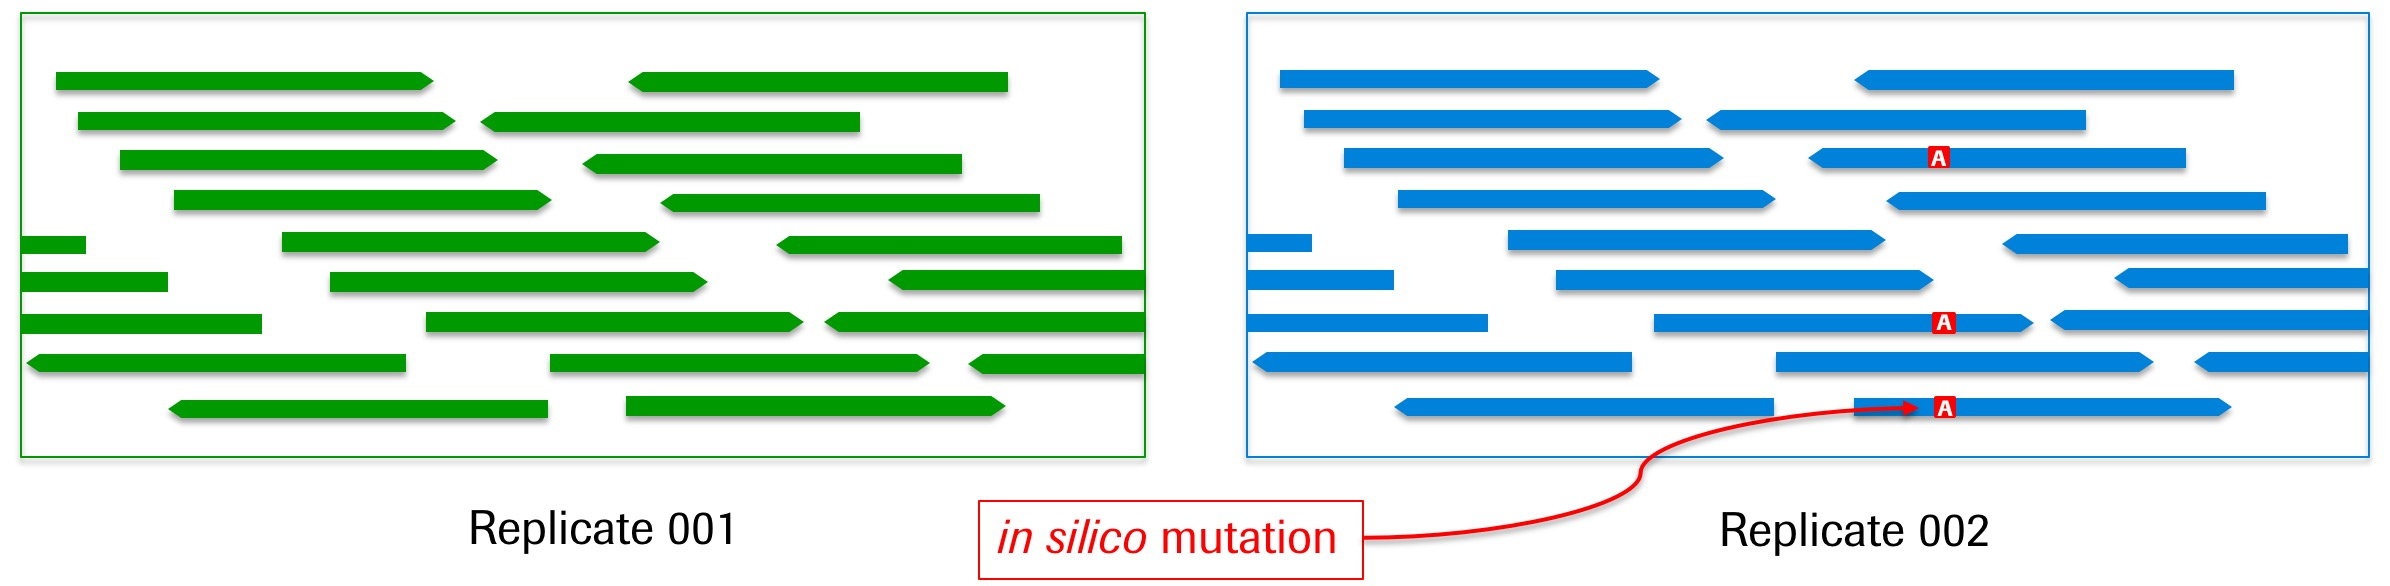
\includegraphics[width=6.5in]{../utilities/dockered_pipelines/bamSimulator/replicate_sim.jpg}
 % replicate_sim.jpg: 2390x586 px, 144dpi, 42.16x10.34 cm, bb=0 0 1195 293
\end{center}





\subsubsection{This example mimicks DREAM Challenge}

\href{https://www.synapse.org/#!Synapse:syn312572/wiki/70726}{DREAM Somatic Mutation Calling Challenge} was an international competition to find algorithms that gave the most accurate performances. 

In that case, a high-coverage BAM file is randomly split into two. One of which is designated normal, and the other one is designated tumor where mutations will be spiked in. Like the previous example, any mutations found between the designated tumor and designated normal are false positive, since not only are they from the same sample, but also from the same sequencing run. This example will not capture false positives as a result of run-to-run biases if they exist in your sequencing data. It will, however, still capture artefacts related to sequencing errors, sampling errors, mapping errors, etc.


\begin{lstlisting}
$PATH/TO/somaticseq/utilities/dockered_pipelines/bamSimulator/BamSimulator_multiThreads.sh \
--genome-reference /ABSOLUTE/PATH/TO/GRCh38.fa --tumor-bam-in /ABSOLUTE/PATH/TO/highCoverageGenome.bam --tumor-bam-out syntheticTumor.bam --normal-bam-out syntheticNormal.bam --split-proportion  0.5 --num-snvs 10000 --num-indels 8000 --num-svs 1500 --min-vaf 0.0 --max-vaf 1.0 --left-beta 2 --right-beta 5 --min-variant-reads 2 --output-dir /ABSOLUTE/PATH/TO/trainingSet --threads 24 --action qsub --split-bam --indel-realign --merge-output-bams
\end{lstlisting}

The --split-bem will randomly split the high coverage BAM file into two BAM files, one of which is designated normal and the other one designated tumor for mutation spike in. The --indel-realign is an option that will perform GATK Joint Indel Realignment on the two BAM files. You may or may not invoke it depending on your real data sets. The --merge-output-bams creates another script that will merge the BAM and VCF files region-by-region. It will need to be run manually after all the spike in is done.

A schematic of the DREAM Challenge simulation procedure

\begin{center}
 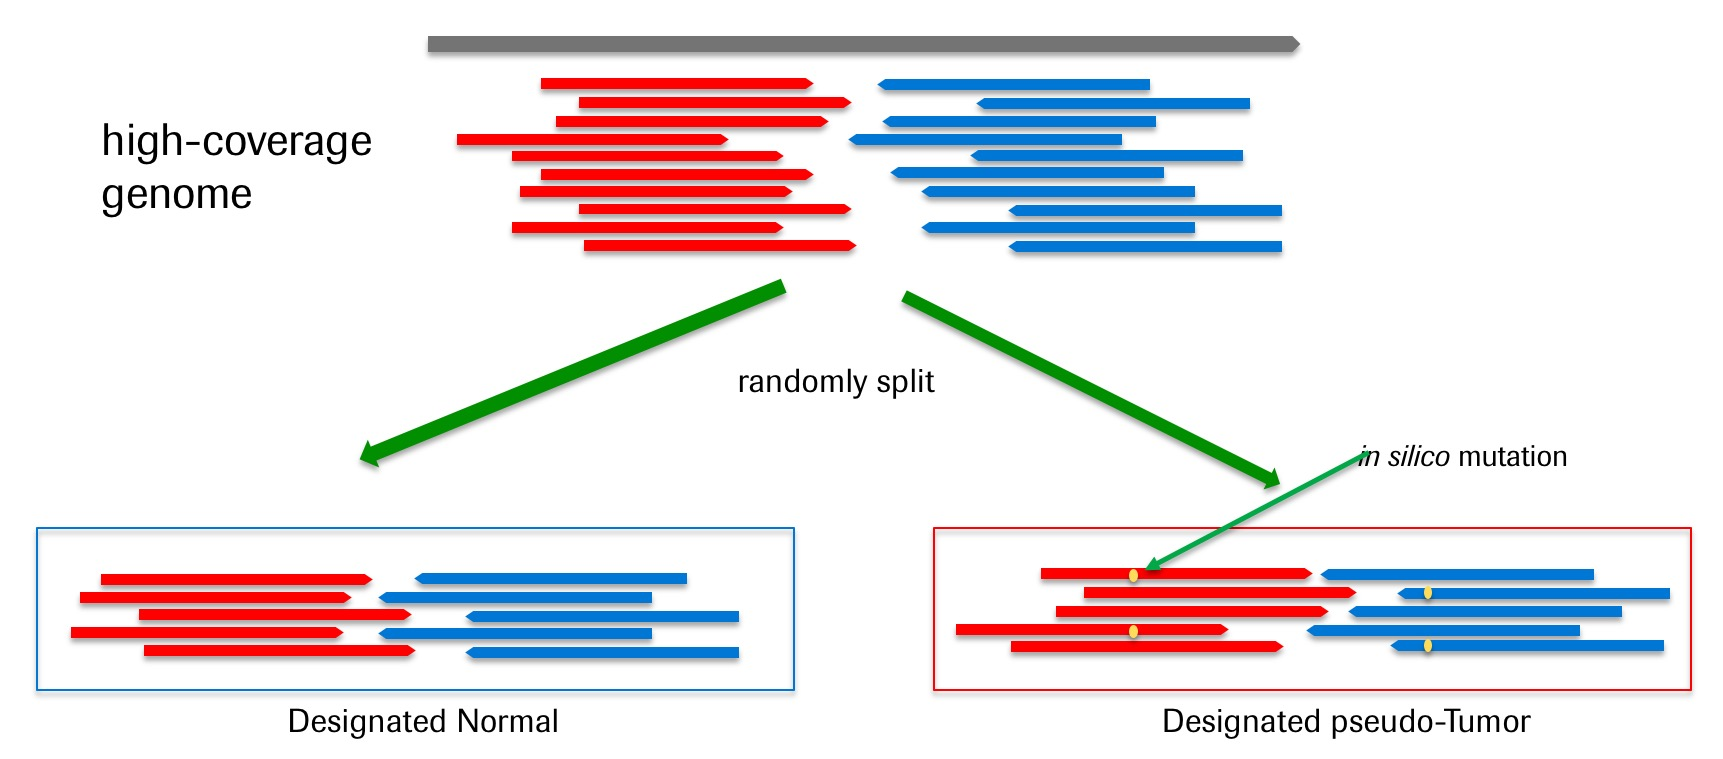
\includegraphics[width=6.5in]{../utilities/dockered_pipelines/bamSimulator/dream_sim.jpg}
 % dream_sim.jpg: 2198x660 px, 144dpi, 38.77x11.64 cm, bb=0 0 1099 330
\end{center}



\subsubsection{Merge and then split the input tumor and normal BAM files}

\begin{lstlisting}
$PATH/TO/somaticseq/utilities/dockered_pipelines/bamSimulator/BamSimulator_multiThreads.sh \
--genome-reference /ABSOLUTE/PATH/TO/GRCh38.fa --tumor-bam-in /ABSOLUTE/PATH/TO/Tumor_Sample.bam --normal-bam-in /ABSOLUTE/PATH/TO/Normal_Sample.bam --tumor-bam-out syntheticTumor.bam --normal-bam-out    syntheticNormal.bam --split-proportion  0.5 --num-snvs 30000 --num-indels 10000 --num-svs 1500 --min-vaf 0.0 --max-vaf 1.0 --left-beta 2 --right-beta 5 --min-variant-reads 2 --output-dir /ABSOLUTE/PATH/TO/trainingSet --threads 24 --action qsub --merge-bam --split-bam --indel-realign --merge-output-bams
\end{lstlisting}

The \textit{\texttt{--}merge-bam} will merge the normal and tumor BAM files into a single BAM file. Then, \textit{\texttt{--}split-bem} will randomly split the merged BAM file into two BAM files. One of which is designated normal, and one of which is designated tumor. Synthetic mutations will then be spiked into the designated tumor to create "real" mutations. This is the approach described in our \href{http://dx.doi.org/10.1158/1538-7445.AM2017-386}{2017 AACR Abstract}.


A schematic of the simulation procedure

\begin{center}
 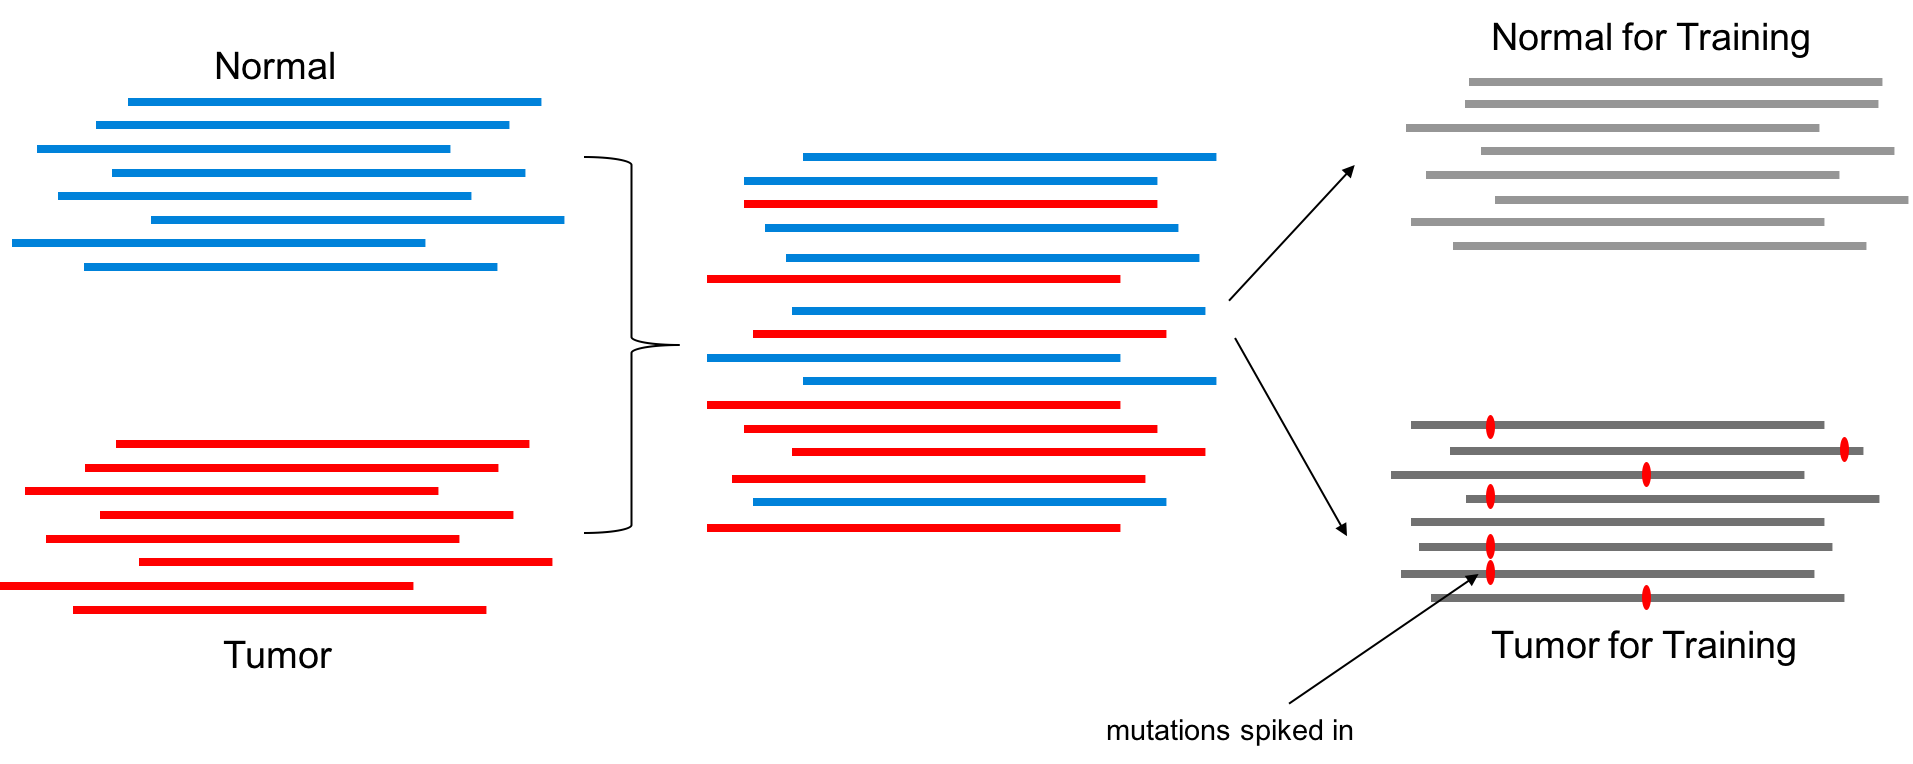
\includegraphics[width=6.5in]{../utilities/dockered_pipelines/bamSimulator/onkoinsight_sim.png}
 % onkoinsight_sim.png: 1913x764 px, 150dpi, 32.39x12.94 cm, bb=0 0 918 367
\end{center}


\subsection{Parameters and Options}

\begin{lstlisting}
--genome-reference  /ABSOLUTE/PATH/TO/human_reference.fa (Required)
--selector          /ABSOLUTE/PATH/TO/capture_region.bed (BED file to limit where mutation spike in will be attempted)
--tumor-bam-in      Input BAM file (Required)
--normal-bam-in     Input BAM file (Optional, but required if you want to merge it with the tumor input)
--tumor-bam-out     Output BAM file for the designated tumor after BAMSurgeon mutation spike in
--normal-bam-out    Output BAM file for the designated normal if --split-bam is chosen
--split-proportion  The faction of total reads desginated to the normal. (Defaut = 0.5)
--num-snvs          Number of SNVs to spike into the designated tumor
--num-indels        Number of INDELs to spike into the designated tumor
--num-svs           Number of SVs to spike into the designated tumor (Default = 0)
--min-depth         Minimum depth where spike in can take place
--max-depth         Maximum depth where spike in can take place
--min-vaf           Minimum VAF to simulate
--max-vaf           Maximum VAF to simulate
--left-beta         Left beta of beta distribution for VAF
--right-beta        Right beta of beta distribution for VAF
--min-variant-reads Minimum number of variant-supporting reads for a successful spike in
--output-dir        Output directory
--merge-bam         Flag to merge the tumor and normal bam file input
--split-bam         Flag to split BAM file for tumor and normal
--clean-bam         Flag to go through the BAM file and remove reads where more than 2 identical read names are present, or reads where its read length and CIGAR string do not match. This was necessary for some BAM files downloaded from TCGA. However, a proper pair-end BAM file should not have the same read name appearing more than twice. Use this only when necessary as it first sorts BAM file by qname, goes through the cleaning procedure, then re-sort by coordinates.
--indel-realign     Conduct GATK Joint Indel Realignment on the two output BAM files. Instead of syntheticNormal.bam and syntheticTumor.bam, the final BAM files will be syntheticNormal.JointRealigned.bam and syntheticTumor.JointRealigned.bam.
--seed              Random seed. Pick any integer for reproducibility purposes.
--threads           Split the BAM files evenly in N regions, then process each (pair) of sub-BAM files in parallel. 
--action            The command preceding the run script created into /ABSOLUTE/PATH/TO/BamSurgeoned_SAMPLES/logs. "qsub" is to submit the script in SGE system. Default = echo
\end{lstlisting}


\subsubsection{--merge-bam / --split-bam / --indel-realign}


If you have sequenced replicate normal, that's the best data set for training. You can use one of the normal as normal, and designate the other normal (of the same sample) as tumor. Use \textit{\texttt{--}indel-realign} to invoke GATK IndelRealign.

When you have a normal that's roughly 2X the coverage as your data of choice, you can split that into two halves. One designated as normal, and the other one designated as tumor. That DREAM Challenge's approach. Use \textit{\texttt{--}split-bam \texttt{--}indel-realign} options.

Another approach is to merge the tumor and normal data, and then randomly split them as described above. When you merge the tumor and normal, the real tumor mutations are relegated as germline or noise, so they are considered false positives, because they are supposed to be evenly split into the designated normal. To take this approach, use \textit{\texttt{--}merge-bam \texttt{--}split-bam \texttt{--}indel-realign options}.

Don't use \textit{\texttt{--}indel-realign} if you do not use indel realignment in your alignment pipeline.

In some BAM files, there are reads where read lengths and CIGAR strings don't match. Spike in will fail in these cases, and you'll need to invoke \textit{\texttt{--}clean-bam} to get rid of these problematic reads.

You can control and visualize the shape of target VAF distribution with python command:

\begin{lstlisting}
    import scipy.stats as stats
    import numpy as np
    import matplotlib.pyplot as plt

    leftBeta, rigthBeta = 2,5
    minAF, maxAF = 0,1
    x = np.linspace(0,1,101)
    y = stats.beta.pdf(x, leftBeta, rigthBeta, loc = minAF, scale = minAF + maxAF)
    _ = plt.plot(x, y)
\end{lstlisting}


\subsection{To create SomaticSeq classifiers}

After the mutation simulation jobs are completed, you may create classifiers with the training data with the following command:

See our \href{https://github.com/bioinform/somaticseq/blob/master/utilities/dockered_pipelines}{somatic mutation pipeline} for more details.

\begin{lstlisting}
makeSomaticScripts.py paired \
--normal-bam           /ABSOLUTE/PATH/TO/trainingSet/syntheticNormal.bam \
--tumor-bam            /ABSOLUTE/PATH/TO/trainingSet/syntheticTumor.bam \
--genome-reference     /ABSOLUTE/PATH/TO/GRCh38.fa \
--output-directory     /ABSOLUTE/PATH/TO/trainingSet/somaticMutationPipeline \
--dbsnp-vcf            /ABSOLUTE/PATH/TO/dbSNP.GRCh38.vcf \
--truth-snv            /ABSOLUTE/PATH/TO/trainingSet/synthetic_snvs.vcf \
--truth-indel          /ABSOLUTE/PATH/TO/trainingSet/synthetic_indels.leftAlign.vcf \
--threads              16 \
--somaticseq-algorithm xgboost \
--train-somaticseq     \
--run-mutect2 --run-vardict --run-muse --run-lofreq --run-strelka2 --run-somaticseq
\end{lstlisting}





\section{Release Notes}

Make sure training and prediction use the same SomaticSeq version, or at least make sure the different minor version changes do not change the results significantly. 


\begin{enumerate}


    \item Version 1.0
    Version used to generate data in the manuscript and \href{https://www.synapse.org/#!Synapse:syn312572/wiki/72943}{Stage 5 of the ICGC-TCGA DREAM Somatic Mutation Challenge}, where SomaticSeq's results were \#1 for INDEL and \#2 for SNV. 

    In the original manuscript, VarDict's var2vcf\_somatic.pl script was used to generate VarDict VCFs, and subsequently ``-filter somatic'' was used for SSeq\_merged.vcf2tsv.py. Since then (including DREAM Challenge Stage 5), VarDict recommends var2vcf\_paired.pl over var2vcf\_somatic.pl, and subsequently ``-filter paired'' was used for SSeq\_merged.vcf2tsv.py. The difference in SomaticSeq results, however, is pretty much negligible. 

    \item Version 1.1
    Automated the SomaticSeq.Wrapper.sh script for both training and prediction mode. No change to any algorithm. 

    \item Version 1.2
    Have implemented the following improvement, mostly for indels:

    \begin{itemize}

      \item 
      SSeq\_merged.vcf2tsv.py can now accept pileup files to extract read depth and DP4 (reference forward, reference reverse, alternate forward, and alternate reverse) information (mainly for indels). Previously, that information can only be extracted from SAMtools VCF. Since the SAMtools or HaplotypeCaller generated VCFs hardly contain any indel information, this option improves the indel model. The SomaticSeq.Wrapper.sh script is modified accordingly.
	    \item
	    Extract mapping quality (MQ) from VarDict output if this information cannot be found in SAMtools VCF (also mostly benefits the indel model). 
	   
	    \item
	    Indel length now positive for insertions and negative for deletions, instead of using the absolute value previously. 
	 
	\end{itemize}
	
	
	
	\item Version 2.0
	
		\begin{itemize}
		  \item
		  Removed dependencies for SAMtools and HaplotypeCaller during feature extraction. SSeq\_merged.vcf2tsv.py extracts those information (plus more) directly from BAM files.
		
		  \item
		  Allow not only VCF file, but also BED file or a list of chromosome coordinate as input format for SSeq\_merged.vcf2tsv.py, i.e., use -mybed or -mypos instead of -myvcf. 
		
		  \item
		  Instead of a separate step to annotate ground truth, that can be done directly by SSeq\_merged.vcf2tsv.py by supplying the ground truth VCF via -truth.
		
		  \item
		  SSeq\_merged.vcf2tsv.py can annotate dbSNP and COSMIC information directly if BED file or a list of chromosome coordinates are used as input in lieu of an annotated VCF file. 
		
		  \item
		  Consolidated feature sets, e.g., removed some redundant features
		  
		  \item
		  Fixed a bug: if JointSNVMix2 is not included, the values should be ``NaN'' instead of 0's. This is to keep consistency with how we handle all other caller decision.
		\end{itemize}
	
	
	
	\item Version 2.0.2
	
		\begin{itemize}
		
		  \item
		  Incorporated LoFreq.
		  
		  \item
		  Used getopt to replace getopts in the SomaticSeq.Wrapper.sh script to allow long options. 
		  
		\end{itemize}
	
	
	
	\item Version 2.1.2
	
	\begin{itemize}
	
	  \item
	  Properly handle cases when multiple ALT's are calls in the same position. The VCF files can either contain multiple calls in the ALT column (i.e., A,G), or have multiple lines corresponding to the same position (one line for each variant call). Some functions were significantly re-written to allow this.
	
	  \item
	  Incorporated Scalpel.
	  
	  \item
	  Deprecated HaplotypeCaller and SAMTools dependencies completely as far as feature generation is concerned.
	  
	  \item
	  The Wrapper script removed SnpSift/SnpEff dependencies. Those information can be directly obtained during the SSeq\_merged.vcf2tsv.py step. Also removed some additional legacy steps that has become useless since v2 (i.e., score\_Somatic.Variants.py). Added a step to check the correctness of the input. The v2.1 and 2.1.1 had some typos in the wrapper script, so only describing v2.1.2 here.
	
	\end{itemize}
	
	
	
	\item Version 2.2
	
		\begin{itemize}
		
		  \item
		  Added MuTect2 support.
		
		\end{itemize}
	
	
	
	\item Version 2.2.1
	
		\begin{itemize}
		
		  \item
		  InDel\_3bp now stands for indel counts within 3 bps of the variant site, instead of exactly 3 bps from the variant site as it was previously (likewise for InDel\_2bp). 
		 
		  \item
		  Collapse MQ0 (mapping quality of 0) reads supporting reference/variant reads into a single metric of MQ0 reads (i.e., tBAM\_MQ0 and nBAM\_MQ0). From experience, the number of MQ0 reads is at least equally predictive of false positive calls, rather than distinguishing if those MQ0 reads support reference or variant. 
		  
		  \item
		  Obtain SOR (Somatic Odds Ratio) from BAM files instead of VarDict's VCF file.
		  
		  \item
		  Fixed a typo in the SomaticSeq.Wrapper.sh script that did not handle inclusion region correctly.
		  
		\end{itemize}
	
	
	
	\item Version 2.2.2
	
		\begin{itemize}
		
		  \item
		  Got around an occasional unexplained issue in then ada package were the SOR is sometimes categorized as type, by forcing it to be numeric. 
		  
		  \item
		  Defaults PASS score from 0.7 to 0.5, and make them tunable in the SomaticSeq.Wrapper.sh script (\texttt{--}pass-threshold and \texttt{--}lowqual-threshold). 
		  
		\end{itemize}
	
	
	
	\item Version 2.2.3
	
		\begin{itemize}
		
		  \item
		  Incorporated Strelka2 since it's now GPLv3.
		  
		  \item
		  Added another R script (ada\_model\_builder\_ntChange.R) that uses nucleotide substitution pattern as a feature. Limited experiences have shown us that it improves the accuracy, but it's not heavily tested yet. 
		
		  \item
		  If a COSMIC site is labeled SNP in the COSMIC VCF file, if\_cosmic and CNT will be labeled as 0. The COSMIC ID will still appear in the ID column. This will not change any results because both of those features are turned off in the training R script.
		  
		  \item
		  Fixed a bug: if JointSNVMix2 is not included, the values should be ``NaN'' instead of 0's. This is to keep consistency with how we handle all other callers.
		  
		\end{itemize}
	
	
	
	\item Version 2.2.4
	
		\begin{itemize}
		
		  \item
		  Resolved a bug in v2.2.3 where the VCF files of Strelka INDEL and Scalpel clash on GATK CombineVariants, by outputting a temporary VCF file for Strelka INDEL without the sample columns.
		  
		  \item
		  Caller classification: consider if\_Scalpel = 1 only if there is a SOMATIC flag in its INFO. 
		
		\end{itemize}
		
		
	
	\item Version 2.2.5
	
		\begin{itemize}
		  
		  \item
		  Added a dockerfile. Docker repo at https://hub.docker.com/r/lethalfang/somaticseq/. 
		  
		  \item
		  Ability to use vcfsort.pl instead of GATK CombineVariants to merge VCF files.
		
		\end{itemize}
	
	
	
	\item Version 2.3.0
	
		\begin{itemize}
		  
		  \item
		  Moved some scripts to the utilities directory to clean up the clutter.
		  
		  \item
		  Added the split\_Bed\_into\_equal\_regions.py to utilities, which will split a input BED file into multiple BED files of equal size. This is to be used to parallelize large WGS jobs.
		  
		  \item
		  Made compatible with MuTect2 from GATK4.
		  
		  \item
		  Removed long options for the SomaticSeq.Wrapper.sh script because it's more readable this way.
		  
		  \item
		  Added a script to add ``GT'' field to Strelka's VCF output before merging it with other VCF files. That was what caused GATK CombineVariants errors mentioned in v2.2.4's release notes. 
		  
		  \item
		  Added a bunch of scripts at utilities/dockered\_pipelines that can be used to submit (requiring Sun Grid Engine or equivalent) dockerized pipeline to a computing cluster. 
		
		\end{itemize}
	
	
	
	\item Version 2.3.1
	
		\begin{itemize}
		
		  \item
		  Improve the automated run script generator at utilities/dockered\_pipelines.
		  
		  \item
		  No change to SomaticSeq algorithm
		
		\end{itemize}
	
	
	
	\item Version 2.3.2
	
		\begin{itemize}
		
		  \item
		  Added run script generators for dockerized BAMSurgeon pipelines at utilities/dockered\_pipelines/bamSurgeon
		  
		  \item
		  Added an error message to r\_scripts/ada\_model\_builder\_ntChange.R when TrueVariants\_or\_False don't have both 0's and 1's. Other than this warning message change, no other change to SomaticSeq algorithm.  
		
		\end{itemize}
	
	
	
	\item Version 2.4.0
	
		\begin{itemize}
		
		  \item
		  Restructured the utilities scripts.
		  
		  \item
		  Added the utilities/filter\_SomaticSeq\_VCF.py script that ``demotes'' PASS calls to LowQual based on a set of tunable hard filters.
		  
		  \item
		  BamSurgeon scripts invokes modified BamSurgeon script that splits a BAM file without the need to sort by read name. This works if the BAM files have proper read names, i.e., 2 and only 2 identical read names for each paired-end reads.
		  
		  \item
		  No change to SomaticSeq algorithm
		
		\end{itemize}
	
	
	
	\item Version 2.4.1
	
		\begin{itemize}
		
		  \item
		  Updated some docker job scripts.
		  
		  \item
		  Added a script that converts some items in the VCF's INFO field into the sample field, to precipitate the need to merge multiple VCF files into a single multi-sample VCF, i.e., utilities/reformat\_VCF2SEQC2.py.
		  
		  \item
		  No change to SomaticSeq algorithm
		
		\end{itemize}
	
	
	
	\item Version 2.5.0
	
		\begin{itemize}
		
		  \item
		  In modify\_VJSD.py, get rid of VarDict's END tag (in single sample mode) because it causes problem with GATK CombineVariants. 
		  
		  \item
		  Added limited single-sample support, i.e., ssSomaticSeq.Wrapper.sh is the wrapper script. singleSample\_callers\_singleThread.sh is the wrapper script to submit single-sample mutation caller scripts.
		  
		  \item
		  Added run scripts for read alignments and post-alignment processing, i.e,. FASTQ $\rightarrow$ BAM, at utilities/dockered\_pipelines/alignments.
		  
		  \item
		  Fixed a bug where the last two CD4 numbers were both alternate concordant reads in the output VCF file, when the last number should've been alternate discordant reads.
		  
		  \item
		  Changed the output file names from Trained.s(SNV$\vert$INDEL).vcf and Untrained.s(SNV$\vert$INDEL).vcf to SSeq.Classified.s(SNV$\vert$INDE).vcf and Consensus.s(SNV$\vert$INDEL).vcf. No change to the actual tumor-normal SomaticSeq algorithm.
		  
		  \item
		  Added utilities/modify\_VarDict.py to VarDict's ``complex'' variant calls (e.g., GCA>TAC) into SNVs when possible. 
		  
		  \item
		  Modified r\_scripts/ada\_model\_builder\_ntChange.R to allow you to ignore certain features, e.g., r\_scripts/ada\_model\_builder\_ntChange.R Training\_Data.tsv nBAM\_REF\_BQ tBAM\_REF\_BQ SiteHomopolymer\_Length ...
		  
		  Everything after the input file are features to be ignored during training.
		  
		  Also added r\_scripts/ada\_cross\_validation.R.
		
		\end{itemize}
	
	
	
	\item Version 2.5.1
	
		\begin{itemize}
		  \item
		  Additional passable parameters options to pass extra parameters to somatic mutation callers. Fixed a bug where the ``two-pass'' parameter is not passed onto Scalpel in multiThreads scripts. 
		  
		  \item
		  Ignore Strelka\_QSS and Strelka\_TQSS for indel training in the SomaticSeq.Wrapper.sh script.
		  
		\end{itemize}
	
	
	
	\item Version 2.5.2
	
		\begin{itemize}
		  \item
		  Ported some pipeline scripts to singularities at utilities/singularities.
		  
		\end{itemize}
	
	
	
	\item Version 2.6.0
	
		\begin{itemize}
		  \item
		  VarScan2\_Score is no longer extracted from VarScan's output. Rather, it's now calculated directly using Fisher's Exact Test, which reproduces VarScan's output, but will have a real value when VarScan2 does not output a particular variant. 
		  
		  \item
		  Incorporate TNscope's output VCF into SomaticSeq, but did not incorporate TNscope caller into the dockerized workflow because we don't have distribution license. 
		  
		\end{itemize}
	
	
	
	\item Version 2.6.1
	
		\begin{itemize}
		  \item
		  Optimized memory for singularity scripts.
		  
		  \item
		  Updated utilities/bamQC.py and added utilities/trimSoftClippedReads.py (removed soft-clipped bases on soft-clipped reads)
		  
		  \item
		  Added some docker scripts at utilities/dockered\_pipelines/QC
		
		\end{itemize}
	
	
	
	\item Version 2.7.0
	
		\begin{itemize}
		  \item
		  Added another feature: consistent/inconsistent calls for paired reads if the position is covered by both forward and reverse reads. However, they're excluded as training features in SomaticSeq.Wrapper.sh script for the time being. 
		  
		  \item
		  Change non-GCTA characters to N in VarDict.vcf file to make it conform to VCF file specifications. 
		
		\end{itemize}
		
		
		\item Version 2.7.1
		
		\begin{itemize}
		
		  \item
		  Without --gatk \$PATH/TO/GenomeAnalysisTK.jar in the SomaticSeq.Wrapper.sh script, it will use utilities/getUniqueVcfPositions.py and utilities/vcfsorter.pl to (in lieu of GATK3 CombineVariants) to combine all the VCF files. 
		
		  \item
		  Fixed bugs in the docker/singularities scripts where extra arguments for the callers are not correctly passed onto the callers. 
		
		\end{itemize}
	
	
	
	\item Version 2.7.2
	
		\begin{itemize}
		
		  \item
		  Make compatible with .cram format
		  
		  \item
		  Fixed a bug where Strelka-only calls are not considered by SomaticSeq. 
		  
		\end{itemize}
	
	
	
	\item Version 2.8.0
	
		\begin{itemize}
		
		  \item
		  The program is now designed to crash if the VCF file(s) are not sorted according to the .fasta reference file. 
		  
		\end{itemize}
	
	
	
	\item Version 2.8.1
	
		\begin{itemize}
		
		  \item
		  Fixed a bug in the ssSomaticSeq.Wrapper.sh script (single-sample mode), where the SNV algorithm weren't looking for SNV VCF files during merging when using utilities/getUniqueVcfPositions.py, causing empty SNV files. For previous commands (invoking --gatk for CombineVariants), the results have never changed. 
		  
		\end{itemize}
	
	
	
	\item Version 3.0.0
	
		Refactored the codes.
		  
			\begin{itemize}
		
		     	\item The wrapper scripts written in bash script (i.e., \textit{SomaticSeq.Wrapper.sh} and \textit{ssSomaticSeq.Wrapper.sh}) are replaced by \textit{somaticseq/run\_somaticseq.py}, though they're still kept for backward-compatibility. 
		     
		    	    \item Allow parallel processing using \textit{somaticseq\_parallel.py}
		
		    \end{itemize}
	
	
	\item Version 3.0.1
		\begin{itemize}
		
		  \item
		  Fixed a bug that didn't handle Strelka/LoFreq indel calls correctly in \textit{somaticseq/combine\_callers.py} module.
		  
		\end{itemize}
	


	\item Version 3.1.0
		\begin{itemize}
		
		  \item
		  When splitting MuTect2 files into SNV and INDEL, make sure either the ref base or the alt base (but not both) consists of a single base, i.e., discarding stuff like GCAA$>$GCT.
		  
		  \item
		  Fixed a bug introduced in v3.0.1 that caused the program to handle .vcf.gz files incorrectly.
		  
          \item
          Incorporated Platypus into paired mode.
		  
		\end{itemize}

		
    \item Version 3.1.1
        \begin{itemize}
         
         \item 
         Fixed some bash scripts involved with single-sample multi-thread callers.
         
         \item
         \textit{vcfModifier/splitVcf.py} to handle multi-allelic calls better for indels. 
         
        \end{itemize}


	\item Version 3.2.0
        \begin{itemize}
         
         \item 
         Re-wrote in Python some somatic caller run script generators that were once written in bash, at \textit{utilities/dockered\_pipelines/makeSomaticScripts.py}. See Section \ref{dockerized_callers} for details. 
         
         \item
         Fixed \textit{setup.py}, even though running \textit{./setup.py install} is optional. You can still run scripts from where you downloaded SomaticSeq. 
 
        \end{itemize}


	\item Version 3.2.1
	
		\begin{itemize}
		
			\item Fixed the TA2CG feature in \textit{ada\_model\_builder\_ntChange.R}.
		
		\end{itemize}


	\item Version 3.3.0
	
		\begin{itemize}

			\item Added support for xgboost (extreme gradient boosting) as an optional substitute for ada (adaptive boosting).
					
			\item Also fixed the TA2CG feature in \textit{ada\_model\_predictor.R}
			
			\item Changed tree depth to 16 in ada model training because internal benchmarking found this to be optimal.
			
			\item Modified \textit{utilities/dockered\_pipelines/create\_tumor\_normal\_run\_scripts.py} and \textit{utilities/dockered\_pipelines/create\_tumor\_only\_run\_scripts.py} to pre-process bed file for VarDict (i.e., limit each line of bed file to 5000 bp) no matter what. Originally the process is triggered if average bp per line was greater than 50,000 bp. That assumption broke down in multi-threaded tasks, when the final sub bed file contained many decoy or non-human contigs that drove the average bp/line in a bed file below 50,000 bp, and the resulting job caused VarDict to run out of memory. This is to rectify that issue.

            \item Occasionally in bamSurgeon workflow, the synthetic\_indels.vcf file will contain non-GCTAN characters in the REF column, causing subsequent GATK LeftAlign to fail. Created the \textit{utilities/dockered\_pipelines/bamSimulator/bamSurgeon/convert\_nonStandardBasesInVcfs.py} script to take care of that. 
		
		\end{itemize}

		
		
	\item Version 3.4.0
	
		\begin{itemize}
            \item Added linguistic sequence complexity (LC) described by Troyanskaya OG \textit{et. al.} as an additional genomic feature \cite{sequence_complexity}. Thus, models trained on this version are not compatible with tsv files created previously becuase it will include a feature not found in previous versions. However, models created from previous version can still be used here. LC is calculated over a 80-bp window spanning the variant site. In addition, LC is also calculated for 80-bp windows on the left and on the right of the variant position, and we record the lower number. The value is converted to Phred in the output. 

            \item Fixed a bug in xgboost mode where training and testing used different feature sets. 

            \item Change ada classifier's file name from *.ntChange.Classifier.RData to *.ada.Classifier.RData to better distinguish them from xgboost. 
		
		\end{itemize}

		
	\item Version 3.4.1
	
		\begin{itemize}
            \item Fixed a bug where indels within 3 bps of a position double-counted indels within 1 bp of the position.
		
		\end{itemize}


	\item Version 3.4.2

        \begin{itemize}
            \item Modified the linguistic sequence complexity calculation to limit the substring to 20-bp. It increases runtime with no sacrifice of accuracy.

            \item Fixed a bug where the indels nearest to a position was not calculated correctly when there are soft-clipped bases in a read.

		\end{itemize}


	\item Version 3.5.0

        \begin{itemize}
            \item Replaced z-scores from scipy's ranksums with p-values from scipy's mannwhitneyu, mostly because the mannwhitneyu corrects for discrete values. Thus, models built prior to this version is no longer compatible with it due to different features. 
		\end{itemize}


	\item Version 3.5.1

        \begin{itemize}
            \item Fixed a minor bug when num\_caller in \textit{somaticseq/somatic\_vcf2tsv.py} and \textit{somaticseq/single\_sample\_vcf2tsv.py} was not reset when there are multiple variant calls in the same genomic position. So, some variant calls that should not be output into the .tsv because num\_caller did not meet the threshold will be output into the .tsv file. However, the features are still reported correctly, so the classifications will still be correct. 

		\end{itemize}

		
	\item Version 3.5.2

        \begin{itemize}
            \item Got around VarDict's latest output VCF file that are incompatible with bedtools by removing the offending lines. Extra steps (may remove later if it becomes unnecessary) were added to somaticseq/combine\_callers.py.
            
            \item Noticed that the xgboost script in R is not compatible with version 1.0+ xgboost library in R.
            
		\end{itemize}
		
    
	\item Version 3.6.0

        \begin{itemize}
            \item Re-wrote the XGBoost routine to use the xgboost library in python (somaticseq/somatic\_xgboost.py), and made it the default algorithm for SomaticSeq because xgboost in python is orders of magnitudes faster than AdaBoost in R. Added dependencies for python's pandas and xgboost libraries. Thus, if you do not intend to use the AdaBoost package in R (it does not support multi-threaded learning and requires large amount of memory), R is not required. To keep using AdaBoost, make sure to invoke \textit{-algo ada}. As a script, \textit{somatic\_xgboost.py} can also be run on its own, with the ability to take in multiple SomaticSeq TSV files. It will combine the TSV files before training (for prediction mode there can only be one input TSV file). Some parametes are also tunable. Run \textit{somatic\_xgboost.py train -h} or \textit{somatic\_xgboost.py predict -h} to see full options. 
            
            \item Remove obsolete \textit{SomaticSeq.Wrapper.sh} and \textit{ssSomaticSeq.Wrapper.sh} scripts. They were obsolete since v3.0.0. 
            
		\end{itemize}
    
		
\end{enumerate}




\section{Contact Us}
For suggestions, bug reports, or technical support, please post in \href{https://github.com/bioinform/somaticseq/issues}{https://github.com/bioinform/somaticseq/issues}. The developers are alerted when issues are created there. Alternatively, you may also email \href{mailto:li_tai.fang@roche.com}{li\_tai.fang@roche.com}. 





%% REFERENCES
\bibliographystyle{unsrt}
\bibliography{Refs}





\end{sloppypar}
\end{document}
